\newpage
\section{Projekt wstępny}
Aby zaprojektować graficzny interfejs użytkownika, wykorzystane zostało narzędzie Figma. Prezentacja makiety kilku ekranów aplikacji znajduje się pod \href{https://www.figma.com/proto/1yxKJbcj7I3atl6e7OpHO8/TravelApp?type=design&node-id=1-247&scaling=min-zoom&page-id=0%3A1&starting-point-node-id=1%3A154}{tym linkiem}.

W projekcie są pokazane przykładowe przejścia między wybranymi ekranami dostępnymi dla użytkownika. Warto wspomnieć że jest to jedynie makieta interfejsu która uległa znacznym zmianom względem wersji finalnej.

\subsection{Ekran logowania}
\begin{figure}[H]
    \centering
    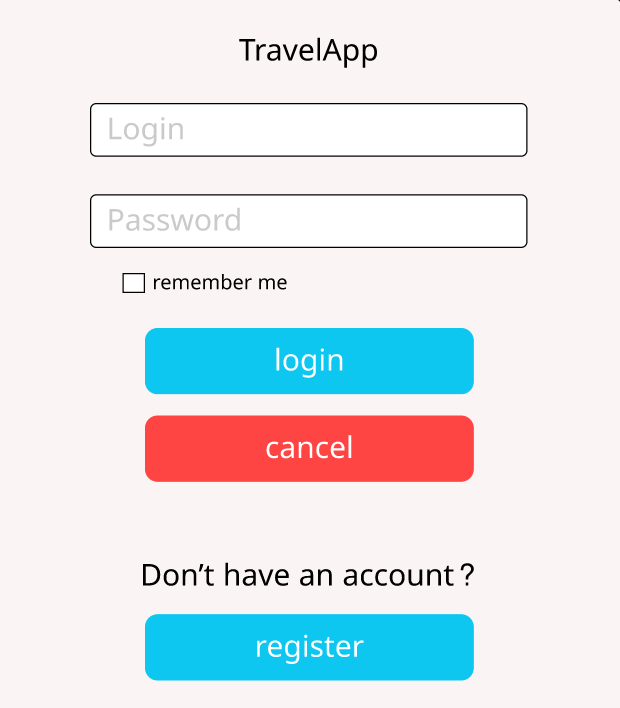
\includegraphics[width=0.5\textwidth]{img/4/logowanie.png}
    \caption{Ekran logowania do aplikacji}
    \label{fig:proj-wstepny-ekran-logowania}
\end{figure}

Na tym ekranie dostępne są dwa pola, do których użytkownik może podać swoje dane potrzebne w celu logowania się do aplikacji jeżeli posiada już konto. W przypadku kiedy konta nie posiada, może wybrać opcję pod przyciskiem "register" która spowoduje pojawienie się nowego ekranu. \\

\subsection{Ekran rejestracji}
\begin{figure}[H]
    \centering
    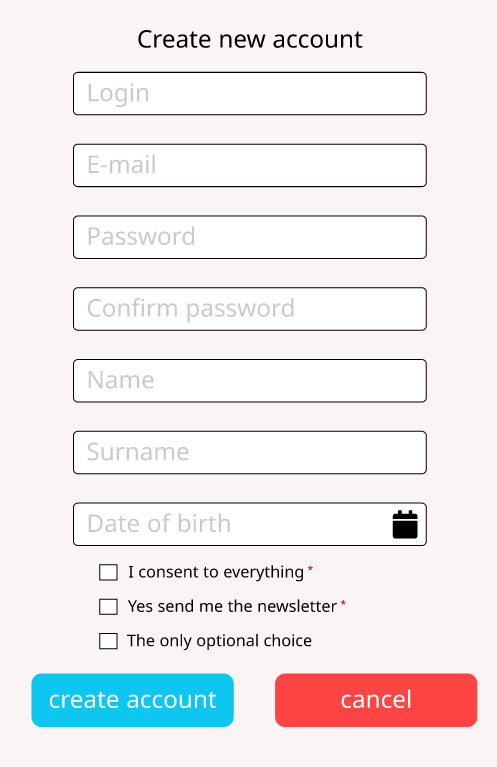
\includegraphics[width=0.5\textwidth]{img/4/rejestracja.png}
    \caption{Ekran rejestracji nowego użytkownika}
    \label{fig:proj-wstepny-ekran-rejestracji}
\end{figure}

Ekran rejestracji przedstawia formularz który użytkownik musi wypełnić w celu założenia nowego konta. Aby to zrobić, wymagane jest podanie loginu który będzie używany przez aplikację do rozpoznawania użytkowników wraz z adresem e-mail, hasłem oraz imieniem i nazwiskiem. Jako ostatnie pole wymagane jest podanie daty urodzenia.
Aby rejestracja mogła zostać ukończona, osoba zakładająca konto musi wyrazić odpowiednie zgody marketingowe i zaakceptować wysyłanie newslettera na podany wcześniej adres mailowy. Jeżeli wszystko zostanie podane, może on użyć przycisku "create account" aby dokończyć proces zakładania konta. W każdej chwili możliwa jest też rezygnacja i powrót do ekranu logowania poprzez wciśnięcie przycisku "cancel".

\subsection{Lista dostępnych atrakcji}
\begin{figure}[H]
    \centering
    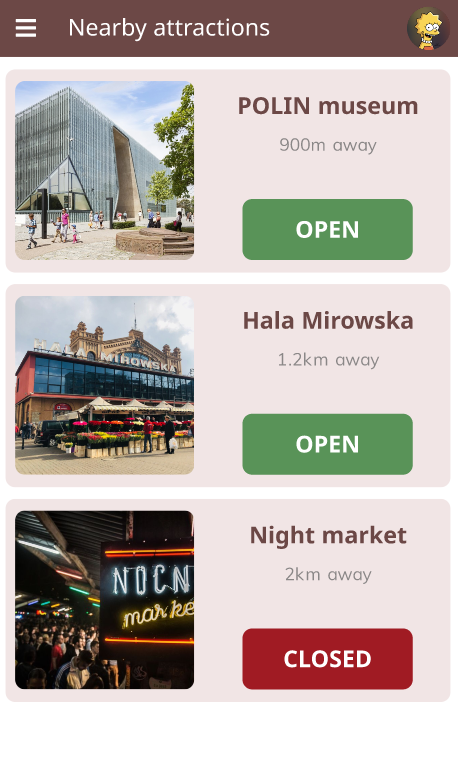
\includegraphics[width=0.5\textwidth]{img/4/lista.png}
    \caption{Ekran z listą dostępnych atrakcji turystycznych}
    \label{fig:proj-wstepny-lista}
\end{figure}

Na tym ekranie użytkownik ma dostępną listę dostępnych atrakcji które znajdują się w jego pobliżu. Lista obiektów posortowana jest względem jego bieżącej pozycji i ponadto podana jest informacja o tym, czy dana atrakcja jest w tej chwili możliwa do zwiedzenia poprzez komunikaty "OPEN" albo "CLOSED" wyświetlane w karcie każdej atrakcji. Podana jest również nazwa obiektu i zdjęcie przedstawiające atrakcję.